\begin{refsection}
\chapter{Screening for chromosomal rearrangements in children with CTHD}
\chaptermark{Screening for chromosomal rearrangements}
%\chapter[HRB and \textit{FMR1} Mutation Screening]{CYTOGENETIC EVALUATION BY HIGH RESOLUTION BANDING AND MOLECULAR GENETIC SCREENING OF \textit{FMR1} GENE MUTATION} % Main chapter title

\label{Chapter3} % For referencing the chapter elsewhere, use \ref{Chapter1}
%thispagestyle{empty}

%----------------------------------------------------------------------------------------

\section{Introduction}
Cytogenetic evaluation of children with CHD and CTHD was made possible by the development of the karyotype in the first half of the 20th century. Some decades later, the introduction of techniques for longitudinal staining of chromosomes, known as banding, and the emergence of techniques for high chromosomal resolution allowed the numerical and structural chromosomal changes to be better recognized and diagnosed. It has been estimated that between 8 and 13\% of all cases of CTHD are associated with microscopically visible chromosomal abnormalities \cite{nora1993causes, ferencz1989congenital}, but this is likely to be an underestimate of the true prevalence. Generally only a subset of individuals with CTHD have their chromosomes analyzed, which is often based on the presence of other organ system anomalies suggestive of a genetic syndrome \cite{nora1993causes, hartman2011contribution, johnson1997chromosome}. As only 25\% to 40\% of patients with CTHD are reported to have other birth anomalies \cite{bernstein2004evaluation, richards2008cryptic}, many individuals are unlikely to have received chromosome analysis. 

By the 1980s, a new concept was created termed as molecular cytogenetics and included techniques of fluorescence in situ hybridization (FISH), spectral karyotyping (SKY), and comparative genomic hybridization (CGH). These new techniques meant that the detection of chromosome abnormalities in CTHD, previously limited to aneuploidies or large rearrangements, could now extend to the identification of complex and very subtle changes, such as microdeletions and microduplications, which may not appear in a standard cyto-genetic analysis. A case in point was the 22q11.2 microdeletion, which accounts for 5\% of all CTHD \cite{zweier2007human}

Studies have identified the 22q11 microdeletion in TOF, TA, IAA, VSD, with a higher prevalence in CTHD with a concurrent aortic arch anomaly \cite{volpe200322q11, momma2010cardiovascular, park2007cardiovascular, ziolkowska2008chromosome, mcdonald2008genetic, mcelhinney2003chromosome, mcelhinney2001association, goldmuntz1998frequency}. In contrast, the 22q11 microdeletion is uncommonly reported in cases with other CTHD such as DORV and TGA \cite{momma2010cardiovascular, goldmuntz1998frequency, van2011changing}. Given the limited size and description of the cases reported in previous studies, it has been difficult to detail the cardiac anatomy associated with a 22q11 microdeletion. 

Since cytogenetic screening of individuals diagnosed with CTHD was the primary step in the inclusion of cases for mutation analysis, chromosomal analysis for both groups and FISH for the 22q11.2 microdeletion for the cases alone was performed. The purpose of the FISH analysis was also to determine which CTHD was more likely to have a 22q11 microdeletion in this study population to better guide clinical screening.


% check ref to chap 2

\section{Methodology}
Phytohemagglutinin stimulated 72 hour lymphocyte cultures of the peripheral blood from the cases (n= 100) and control (n=100) groups were processed and Giemsa banded by methods outlined in Section 2.3.1. For each subject, 25 metaphases with chromosomes at a 450-550 band resolution were examined for any structural or numerical abnormalities. 
Subsequently, FISH was performed using a dual colour commercial probe (Vysis© DiGeorge Region Probe-LSI \textit{TUPLE1} Spectrum-orange/LSI \textit{ARSA} Spectrum-green) that results in the simultaneous labeling of the \textit{TUPLE1} gene and a control terminal region \textit{ARSA} of chromosome 22. FISH was performed on fixed metaphases of the cases that had a normal karyotype, as detailed in Section 2.3.2


\section{Results}

\subsection*{Chromosomal abnormalities and variations}


While cytogenetic analysis of the 100 controls revealed neither numerical nor structural chromosomal anomalies, abnormalities were observed in three cases (\cref{fig:KT3.1}, \cref{fig:KT3.2} and \cref{fig:KT3.3}) presenting with TOF (\cref{tab:3.1abnormalkt}).

In addition to the well defined abnormalities, a few chromosomal variations in some of the cases were noted. This included additional heterochromatin in chromosome 9 (9qh+)in 3\%, additional heterochromatin in chromosome Y (Yqh+) in 1\% and large satellites in chromosome 15,21 and 22 ,each in 1\% of the cases . However these were considered to be normal variants often seen in the general population with no reported clinical significance.

\begin{landscape}
\begin{table}[!p]
\centering
\caption{Details of cases detected with a chromosomal abnormality}
\label{tab:3.1abnormalkt}
\begin{tabular}{p{0.75in}  p{2.15in}  p{0.75in}  p{5in}  }
\hline
	Case ID & Chromosomal abnormality &  Age/Gender &  Family and clinical history \\ \hline
	CTHD\#53 & 46,XX,t(5;19)(p13.1;q14)pat & 4y/F & First born of a non-consanguineous marriage. In addition to TOF, features of small for gestational age, microcephaly, hypertelorism, broad nasal bridge, abnormal auricle, operated cleft lip, single palmar crease and flat feet and hypertonia of all limbs were noted   \\ \hline
	CTHD\#73 & 46,XY,der(17)add(q24) & 1y/M & First born of a non-consanguineous marriage. In addition to TOF, he had development delay and frequent seizures. Parental karyotyping was not possible as they did not consent. \\ \hline
	CTHD\#78 & 47,XY,+22,del(22)(q13.1→qter) & NB/M & First born of a non-consanguineous marriage. In addition to TOF, he had generalized cyanosis, respiratory distress and bradycardia and severe growth retardation. Congenital anomalies which included microcephaly, hypertelorism, low-set ears, bilateral complete cleft lip and palate, micrognathia, clenched hands, cryptorchidism, and penoscrotal hypospadias were also observed. Parental karyotyping was not possible as they did not consent. \\ \hline
	
\end{tabular}
\end{table}
\end{landscape}

\begin{figure}[!thbp]
\centering
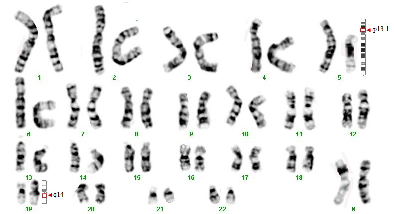
\includegraphics[width=\linewidth]{Figures/Figure3_1.pdf}
\rule{35em}{0.5pt}
\caption{Representative karyotype of the patient with 46,XX,t(5;19)(p13.1;q14)pat [CTHD\#53]}
\label{fig:KT3.1}
\end{figure}

\begin{figure}[!thbp]
\centering
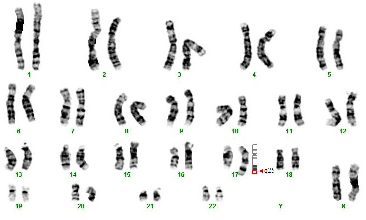
\includegraphics[width=\linewidth]{Figures/Figure3_2.pdf}
\rule{35em}{0.5pt}
\caption{Representative karyotype of the patient with 46,XX,der(17)add(q25) [CTHD\#73]}
\label{fig:KT3.2}
\end{figure}

\begin{figure}[!thbp]
\centering
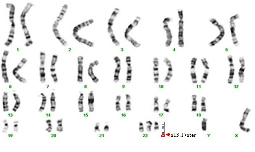
\includegraphics[width=\linewidth]{Figures/Figure3_3.pdf}
\rule{35em}{0.5pt}
\caption{Representative karyotype of the patient with 47,XY,+22,del(22)(q13.1→qter) [CTHD\#78]}
\label{fig:KT3.3}
\end{figure}

The distribution of chromosomal abnormalities between the two groups, calculated by Fisher’s exact test, was not statistically significant (p < 0.05). The difference in the male to female ratio between the two groups was also not statistically significant.

\subsection*{FISH analysis}
FISH analysis revealed 1 of the 100 cases to have the deletion at the 22q11.2 locus (\cref{fig:FISH3.4}). The frequency of the 22q11.2 micro-deletion in the subjects carrying CTHD with and/or without extracardiac signs was thus estimated to be 1\%. However, when analyzing the groups separately, the deletion was present in none of the patients with isolated conotruncal heart defect. 

\begin{figure}[!tb]
\centering
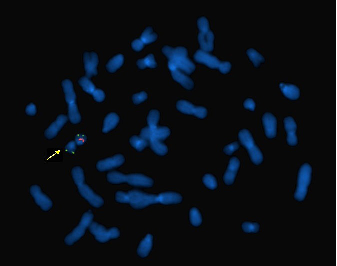
\includegraphics[width=\linewidth]{Figures/Figure3_4.pdf}
\rule{35em}{0.5pt}
\caption{Representative metaphase of the patient with the 22q11.2 deletion detected by FISH.
The red signal indicates the 22q11.2 (\textit{TUPLE1}) region and the green signal the terminal chromosome 22(\textit{ARSA}) control region.
The arrow indicates the deleted chromosome 22, showing the presence of the control region only.}
\label{fig:FISH3.4}
\end{figure}

The micro-deleted proband was a male and the first child of a non- consanguineous marriage, His age at the time of diagnosis was 1 year 6 months and the echocardiocagraphy showed a confluent PA, right aortic arch, large misaligned subaortic VSD with infundibular and valva PS. The extracardiac features included a small chin, hooded eyelids, narrow palbebral fissure, rectangular nose, abnormal ears. Unfortunately , the immunological status of the child was not evaluated at the time of the study.



\section{Discussion} \label{18deldup}

Around 15 to 20\% of cases with CTHD present with a chromosomal abnormality identified by karyotyping \cite{robinson1994clinical, blue2012congenital}. Depending on the abnormality observed, there may also be the need for assessment of other family members and a higher recurrence risk in the offspring which highlights the importance of performing this investigation for this population \cite{hartman2011contribution, harris2003epidemiology, stoll1989risk, pradat1992epidemiology, hanna1994genetic, goodship1998population, grech1999syndromes, meberg2000outcome, roodpeyma2002risk, calzolari2003congenital, dadvand2009descriptive, hartman2011contribution, rosa2011trisomy}.

In this series, three patients who had been diagnosed with TOF had a structural chromosomal abnormality. For case CTHD058 the rearrangement was determined to be paternally inherited while for other two cases, 73 and 78, the origin of the rearrangement could not be established since parental karyotyping was not possible.. No numerical abnormalities were observed. This was an expected result since CTHD associated with numeric chromosomal abnormalities, in general trisomies, are seen within a well determined syndromic framework, which was not the case in this study population. As seen in \cref{tab:3.2litreview}, the frequency of reported abnormalities when compared to other similar studies was low, and this was largely attributed to the selection criteria of the cases. A majority of the cases were non-syndromic CTHD (74\%) with only a small percentage (26\%) having extra-cardiac features suggestive of a chromosomal syndrome. 

Patients with chromosomal abnormalities often have associated extra-cardiac malformations, and are therefore at a higher risk of morbidity and mortality \cite{hanna1994genetic, marino2000congenital, begic2003epidemiological, gonzalez2009universal}. Therefore it is important to establish an accurate diagnosis of the etiology of CTHD since families need genetic counseling with accurate information about the risks of recurrence \cite{prasad2002genetics}. In cases of numerical abnormalities by full trisomy or total monosomy of a chromosome, there is no indication of parental karyotype assessment, because those are usually due to errors that occur during gametogenesis.

On the other hand, in cases of structural abnormalities, such as deletions and duplications, there is always an indication for a parental karyotype, in order to rule out the possibility that one of them carries a balanced chromosomal abnormality related to that observed in the child. 

However, it is worth mentioning that the result of a traditional karyotype test does not exclude the fact that the case might still present a cytogenetic abnormality syndrome. Microscopic changes, such as microdeletions or microduplications, are not detected by this test. In fact, only high-resolution techniques (coupled in particular with GTG banding) can make it possible to reveal these expected microrearrangements. These techniques are rather laborious, requiring synchronization stages. They were not adopted in this study as the wish was to search for the 22q11.2 microdeletion in particular by adopting the FISH technique, which is more specific, more sensitive, and targeted.

\begin{landscape}
\begin{table}[!p]
\centering
\caption{Comparison between different studies described in the literature}
\label{tab:3.2litreview}
\begin{tabular}{  P{1in} P{1in} P{2in} P{2in} P{2in}  }
\hline
	Authors & Number of cases studied & Total chromosomal abnormality (\%) & Numeric changes (\%) & Structural changes (\%) \\ \hline
	\cite{ferencz1989congenital} & 2102 & 12.9 & 95.6 & 4.4 \\ \hline
	\cite{harris2003epidemiology} & 12932 & 18 & 92.2 & Not described \\ \hline
	\cite{stoll1989risk} & 801 & 9 & 95.8 & 4.2 \\ \hline
	\cite{pradat1992epidemiology} & 1605 & 13 & Not described & Not described \\ \hline
	\cite{hanna1994genetic} & 388 & 3 & Not described & Not described \\ \hline
	\cite{goodship1998population} & 207 & 12.1 & 90.5 & 9.5 \\ \hline
	\cite{grech1999syndromes} & 231 & 9 & 95.2 & 4.8 \\ \hline
	\cite{meberg2000outcome} & 360 & 6.7 & 83.3 & 16.7 \\ \hline
	\cite{roodpeyma2002risk} & 346 & 9 & 100 & 0 \\ \hline
	\cite{calzolari2003congenital} & 1549 & 9.8 & 86.8 & Not described \\ \hline
	\cite{dadvand2009descriptive} & 5715 & 11.6 & Not described & Not described \\ \hline
	\cite{hartman2011contribution} & 4430 & 10.8 & 89.2 & 10.8 \\ \hline
	\cite{rosa2011trisomy} & 204 & 14 & 88.5 & 11.5 \\ \hline
	\textbf{Present Study} & \textbf{100} & \textbf{3} & \textbf{0} & \textbf{100} \\ \hline
\end{tabular}
\end{table}
\end{landscape}


FISH analysis revealed the 22q11.2 microdeletion in one case. The frequency of the 22q11.2 microdeletion in CTHD was thus estimated at 1\%.This frequency is far lower than the figures reported in the literature \cite{goldmuntz1993microdeletions, iserin1998prevalence}. It should be noted that in most studies relating to the evaluation of the 22q11.2 microdeletion prevalence, the adopted technique is the one used in this study: targeted FISH using the commercial \textit{TUPLE1} probes. It is only in some rare studies that other probes of the type YAC, BAC, or CAP (complementary of particular sequences of the 22q11.2 area) were used \cite{iserin1998prevalence}. According to the series of the Goldmuntz team in Philadelphia, which is the reference team as regards CHD genetics, the frequency of the 22q11.2 microdeletion in subjects carrying non-syndromic CTHD varied from 18\% to 29\% \cite{goldmuntz1993microdeletions}. The selection criteria of the patients were dominated by the major criterion, which was the presence of CTHD. 
The frequency can also vary depending on the type of the CTHD and the age group studied. In a study of Iserin and colleagues, \cite{iserin1998prevalence} the 22q11.2 microdeletion was described in 41\% of TA, 89\% of IAA and 34.5\% TOF. Also, it was shown that the frequency of the 22q11.2 microdeletion was particularly higher in patients showing CTHD explored in the neonatal period.

The rather low figure found in our series could thus be explained on the one hand by the heterogeneity of the age groups and, on the other hand, by the heterogeneity of the clinical presentation. These two factors were inevitable in the study because the selection of the patients was dependent on the scarcity of these pathologies, the prospective and monocentric character of the study, as well as the limited duration of the patient collection. Furthermore, the isolated and/or syndromic character of the CTHD was sometimes difficult to specify, more especially as certain clinical signs such as neonatal hypocalcemia, the immunological checkup centered on the study of T lymphocytes, as well as the radiological aspect of the thymus were not always easy to check. Furthermore, the representation of the various CTHD was heterogeneous in our series, with an over-representation of TOF and a very weak representation of IAA.

In conclusion, despite our results, it appears that chromosomal abnormalities and the 22q11.2 microdeletion could be a frequent etiologic factor of the CTHD, thus possibly justifying its application in the systematic search of any individual carrying a CTHD. Moreover, the frequency of the 22q11.2 microdeletion increases when the CTHD is associated with other evocative signs of the 22q11 microdeletion phenotype. 


\cleardoublepage
\printbibliography[heading=subbibintoc]
\end{refsection}
